\section{Scales}

A scale is a collection of notes in ascending order between a note and its octave. The two main scales are the major (happy sound) and minor (sad sound) scale.

When describing scales, often the terms "whole" (w) and "half" (h) steps are used. Sometimes you will also see the terms "tone" (T) and "semitone" (S). Moving up a half step on the ukulele means moving to the next fret (towards the body). Moving up a whole step is the same as two half steps.

Lets look at the intervals again (\autoref{tab:ukulele_sharp_flat_intervals_chap_5}). Going one step to the left or to the right is a half step interval. To take a whole step, simply take two half steps.

\begin{table}[h]
	\centering
	\begin{tabular}{*{12}{P{5mm}}}
		\large{A} & \large{A\sharp} & \large{B} & \large{C} & \large{C\sharp} & \large{D} & \large{D\sharp} & \large{E} & \large{F} & \large{F\sharp} & \large{G} & \large{G\sharp} \\ \\
		\large{A} & \large{B\flat} & \large{B} & \large{C} & \large{D\flat} & \large{D} & \large{E\flat} & \large{E} & \large{F} & \large{G$\flat$}& \large{G} & \large{A\flat}
	\end{tabular}
	\caption{Sharp and flat intervals. Each step to the left or right is a half step.}
	\label{tab:ukulele_sharp_flat_intervals_chap_5}
\end{table}

\subsection{The major scale}

As mentioned. The most common scales are the major and minor scales. A lot of music theory is based on the major diatonic scale. A diatonic scale means that it has 7 different notes in the scale where each letter only occurs once. So the major diatonic scale is the first one we will learn.

Each scale has a formula. For the major diatonic scale the formula is shown in (\autoref{tab:ukulele_major_scale_interval}). On the top you see the steps between each note (the formula itself). The numbers indicate the index of the note in the scale. Index 1 and 8 are the same note. But index 8 is one octave higher than index 1.

\begin{table}[h]
	\centering
	\begin{tabular}{*{16}{c}}
		& \multicolumn{2}{P{4mm}}{\large{W}} & \multicolumn{2}{P{4mm}}{\large{W}} & \multicolumn{2}{P{4mm}}{\large{H}} & \multicolumn{2}{P{4mm}}{\large{W}} & \multicolumn{2}{P{4mm}}{\large{W}} & \multicolumn{2}{P{4mm}}{\large{W}} & \multicolumn{2}{P{4mm}}{\large{H}} & \\
		\multicolumn{2}{P{4mm}}{1} & \multicolumn{2}{P{4mm}}{2} & \multicolumn{2}{P{4mm}}{3} & \multicolumn{2}{P{4mm}}{4} & \multicolumn{2}{P{4mm}}{5} & \multicolumn{2}{P{4mm}}{6} & \multicolumn{2}{P{4mm}}{7} & \multicolumn{2}{P{4mm}}{8}
	\end{tabular}
	\caption{Major scale intervals}
	\label{tab:ukulele_major_scale_interval}
\end{table}

Note that \autoref{tab:ukulele_sharp_flat_intervals_chap_5} has 12 different notes/pitches. Now count the total amount of half steps that are shown in \autoref{tab:ukulele_major_scale_interval} (a whole step is two half steps). Indeed, there are 12 half steps to go from the note at index 1 to the same note one octave higher (index 8).

To create the C major scale we will start on the C and then simply follow the formula.

\begin{table}[h]
	\centering
	\begin{tabular}{*{16}{c}}
		& \multicolumn{2}{P{4mm}}{\large{W}} & \multicolumn{2}{P{4mm}}{\large{W}} & \multicolumn{2}{P{4mm}}{\large{H}} & \multicolumn{2}{P{4mm}}{\large{W}} & \multicolumn{2}{P{4mm}}{\large{W}} & \multicolumn{2}{P{4mm}}{\large{W}} & \multicolumn{2}{P{4mm}}{\large{H}} & \\
		\multicolumn{2}{P{4mm}}{1} & \multicolumn{2}{P{4mm}}{2} & \multicolumn{2}{P{4mm}}{3} & \multicolumn{2}{P{4mm}}{4} & \multicolumn{2}{P{4mm}}{5} & \multicolumn{2}{P{4mm}}{6} & \multicolumn{2}{P{4mm}}{7} & \multicolumn{2}{P{4mm}}{8} \\
		\multicolumn{2}{P{4mm}}{C} & \multicolumn{2}{P{4mm}}{D} & \multicolumn{2}{P{4mm}}{E} & \multicolumn{2}{P{4mm}}{F} & \multicolumn{2}{P{4mm}}{G} & \multicolumn{2}{P{4mm}}{A} & \multicolumn{2}{P{4mm}}{B} & \multicolumn{2}{P{4mm}}{C}
	\end{tabular}
	\caption{C major scale}
	\label{tab:ukulele_c_major_scale}
\end{table}

\newpage

The G major scale is shown below in (\autoref{tab:ukulele_g_major_scale}).

\begin{table}[h]
	\centering
	\begin{tabular}{*{16}{c}}
		& \multicolumn{2}{P{4mm}}{\large{W}} & \multicolumn{2}{P{4mm}}{\large{W}} & \multicolumn{2}{P{4mm}}{\large{H}} & \multicolumn{2}{P{4mm}}{\large{W}} & \multicolumn{2}{P{4mm}}{\large{W}} & \multicolumn{2}{P{4mm}}{\large{W}} & \multicolumn{2}{P{4mm}}{\large{H}} & \\
		\multicolumn{2}{P{4mm}}{1} & \multicolumn{2}{P{4mm}}{2} & \multicolumn{2}{P{4mm}}{3} & \multicolumn{2}{P{4mm}}{4} & \multicolumn{2}{P{4mm}}{5} & \multicolumn{2}{P{4mm}}{6} & \multicolumn{2}{P{4mm}}{7} & \multicolumn{2}{P{4mm}}{8} \\
		\multicolumn{2}{P{4mm}}{G} & \multicolumn{2}{P{4mm}}{A} & \multicolumn{2}{P{4mm}}{B} & \multicolumn{2}{P{4mm}}{C} & \multicolumn{2}{P{4mm}}{D} & \multicolumn{2}{P{4mm}}{E} & \multicolumn{2}{P{4mm}}{F\sharp} & \multicolumn{2}{P{4mm}}{G}
	\end{tabular}
	\caption{G major scale}
	\label{tab:ukulele_g_major_scale}
\end{table}

In \autoref{tab:ukulele_natural_note_major_scale} you see the major scales of all the natural notes. You don't need to remember these by heart at the moment. You do need to learn the formula of the major scale by heart. There are three things to note:

\begin{enumerate}
	\item Each scale only has unique letters. Therefore the 4th note in the F major scale is a B$\flat$ and not an A$\sharp$.
	\item The 5th note in the scale is the start of the scale on the next row. Of course, this is because they are listed as such now. But it is the basis of the "circle of fifths" which we will learn more about later.
	\item Each scale below another in this list has one more $\sharp$ than the previous. And the notes that have a sharp in one scale, also have sharp in the scales below it. Again, this has to do with the "circle of fifths".
\end{enumerate}

\begin{table}[h]
	\centering
	\begin{tabular}{*{16}{c}}
		& \multicolumn{2}{P{4mm}}{\large{W}} & \multicolumn{2}{P{4mm}}{\large{W}} & \multicolumn{2}{P{4mm}}{\large{H}} & \multicolumn{2}{P{4mm}}{\large{W}} & \multicolumn{2}{P{4mm}}{\large{W}} & \multicolumn{2}{P{4mm}}{\large{W}} & \multicolumn{2}{P{4mm}}{\large{H}} & \\
		\multicolumn{2}{P{4mm}}{1} & \multicolumn{2}{P{4mm}}{2} & \multicolumn{2}{P{4mm}}{3} & \multicolumn{2}{P{4mm}}{4} & \multicolumn{2}{P{4mm}}{5} & \multicolumn{2}{P{4mm}}{6} & \multicolumn{2}{P{4mm}}{7} & \multicolumn{2}{P{4mm}}{8} \\
		\multicolumn{2}{P{4mm}}{F} & \multicolumn{2}{P{4mm}}{G} & \multicolumn{2}{P{4mm}}{A} & \multicolumn{2}{P{4mm}}{B\flat} & \multicolumn{2}{P{4mm}}{C} & \multicolumn{2}{P{4mm}}{D} & \multicolumn{2}{P{4mm}}{E} & \multicolumn{2}{P{4mm}}{F} \\
		\multicolumn{2}{P{4mm}}{C} & \multicolumn{2}{P{4mm}}{D} & \multicolumn{2}{P{4mm}}{E} & \multicolumn{2}{P{4mm}}{F} & \multicolumn{2}{P{4mm}}{G} & \multicolumn{2}{P{4mm}}{A} & \multicolumn{2}{P{4mm}}{B} & \multicolumn{2}{P{4mm}}{C} \\
		\multicolumn{2}{P{4mm}}{G} & \multicolumn{2}{P{4mm}}{A} & \multicolumn{2}{P{4mm}}{B} & \multicolumn{2}{P{4mm}}{C} & \multicolumn{2}{P{4mm}}{D} & \multicolumn{2}{P{4mm}}{E} & \multicolumn{2}{P{4mm}}{F\sharp} & \multicolumn{2}{P{4mm}}{G} \\
		\multicolumn{2}{P{4mm}}{D} & \multicolumn{2}{P{4mm}}{E} & \multicolumn{2}{P{4mm}}{F\sharp} & \multicolumn{2}{P{4mm}}{G} & \multicolumn{2}{P{4mm}}{A} & \multicolumn{2}{P{4mm}}{B} & \multicolumn{2}{P{4mm}}{C\sharp} & \multicolumn{2}{P{4mm}}{D} \\
		\multicolumn{2}{P{4mm}}{A} & \multicolumn{2}{P{4mm}}{B} & \multicolumn{2}{P{4mm}}{C\sharp} & \multicolumn{2}{P{4mm}}{D} & \multicolumn{2}{P{4mm}}{E} & \multicolumn{2}{P{4mm}}{F\sharp} & \multicolumn{2}{P{4mm}}{G\sharp} & \multicolumn{2}{P{4mm}}{A} \\
		\multicolumn{2}{P{4mm}}{E} & \multicolumn{2}{P{4mm}}{F\sharp} & \multicolumn{2}{P{4mm}}{G\sharp} & \multicolumn{2}{P{4mm}}{A} & \multicolumn{2}{P{4mm}}{B} & \multicolumn{2}{P{4mm}}{C\sharp} & \multicolumn{2}{P{4mm}}{D\sharp} & \multicolumn{2}{P{4mm}}{E} \\
		\multicolumn{2}{P{4mm}}{B} & \multicolumn{2}{P{4mm}}{C\sharp} & \multicolumn{2}{P{4mm}}{D\sharp} & \multicolumn{2}{P{4mm}}{E} & \multicolumn{2}{P{4mm}}{F\sharp} & \multicolumn{2}{P{4mm}}{G\sharp} & \multicolumn{2}{P{4mm}}{A\sharp} & \multicolumn{2}{P{4mm}}{B}
	\end{tabular}
	\caption{Major scales of all natural notes}
	\label{tab:ukulele_natural_note_major_scale}
\end{table}

\newpage

In \autoref{fig:ukulele_major_scale_fretboard} different shapes are shown on how the major scale can be played. These shapes can be moved up and down the fretboard, as long as the distance between the frets stay the same. Shape \autoref{fig:ukulele_major_scale_fretboard_single_string} can even be moved up and down the strings. By moving the shape, you will play a different major scale. The scale that you are playing is determined by the root note (the "1" note). In this example we are therefore playing the C$\sharp$ major scale.

There are other "shapes" to play the major scale as well, but these shapes don't start or the root (1) note. We will come back to those later.

Learning these shapes by heart makes it easy to improvise over a song. But more important is to see how these shapes relate to the intervals of the major scale. The easiest shape for this is \autoref{fig:ukulele_major_scale_fretboard_single_string}. With this shape you can easily recognize the major diatonic scale formula (w-w-h-w-w-w-h). All shapes have the same notes, just played on a different position on the fretboard.

\begin{figure}[h]
	\begin{subfigure}[b]{0.45\textwidth}
		\centering
		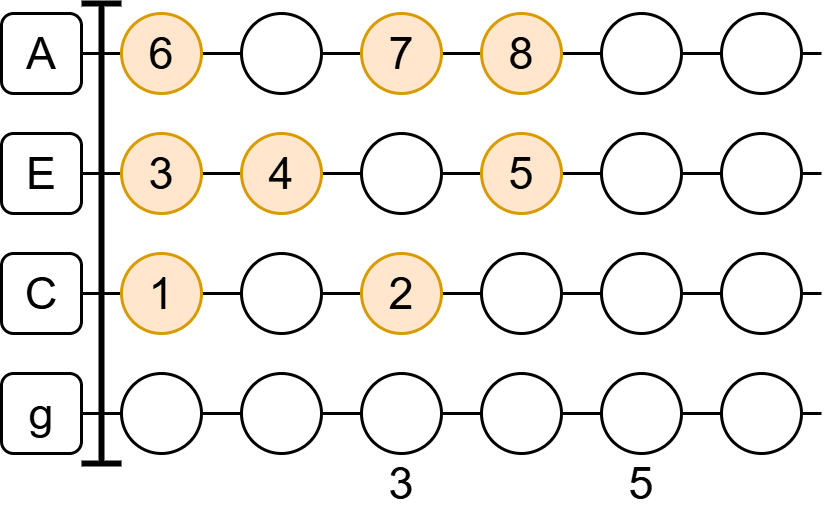
\includegraphics[width=\textwidth]{../../Images/ukulele_major_scale_compact.png}
		\caption{Major scale on the fretboard (shape 1)}
		\label{fig:ukulele_major_scale_fretboard_compact}
	\end{subfigure}
	\hfill
	\begin{subfigure}[b]{0.45\textwidth}
		\centering
		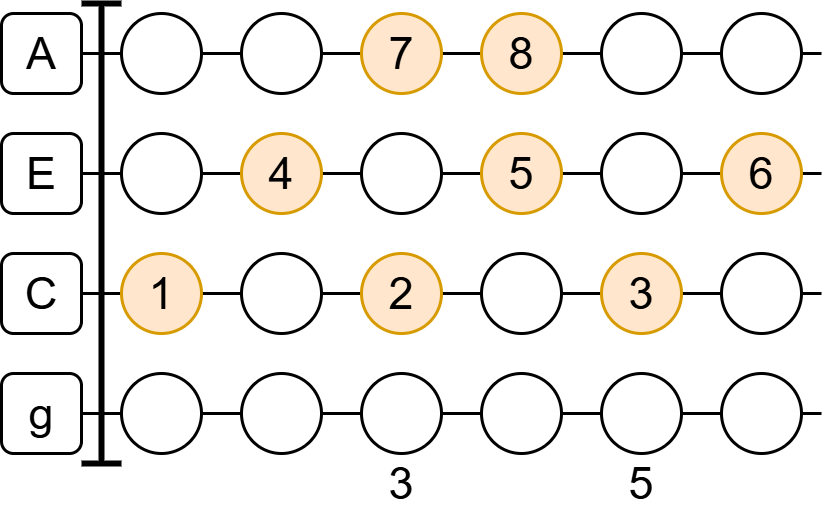
\includegraphics[width=\textwidth]{../../Images/ukulele_major_scale.png}
		\caption{Major scale on the fretboard (shape 2)}
		\label{fig:ukulele_major_scale_fretboard_alt}
	\end{subfigure}
	
	\vspace{0.5cm}
	\begin{subfigure}[b]{\textwidth}
		\centering
		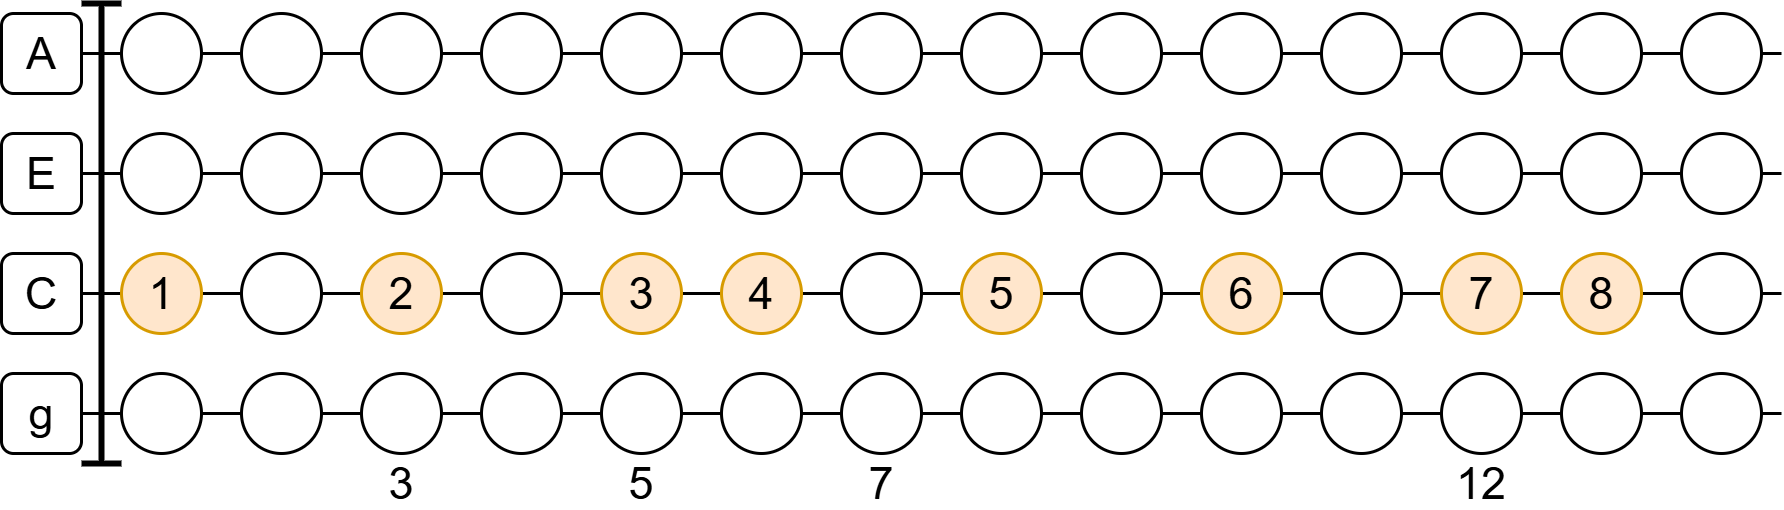
\includegraphics[width=\textwidth]{../../Images/ukulele_major_scale_single_string.png}
		\caption{Major scale on the fretboard on a single string}
		\label{fig:ukulele_major_scale_fretboard_single_string}
	\end{subfigure}
	
	\vspace{0.5cm}
	\begin{subfigure}[b]{\textwidth}
		\centering
		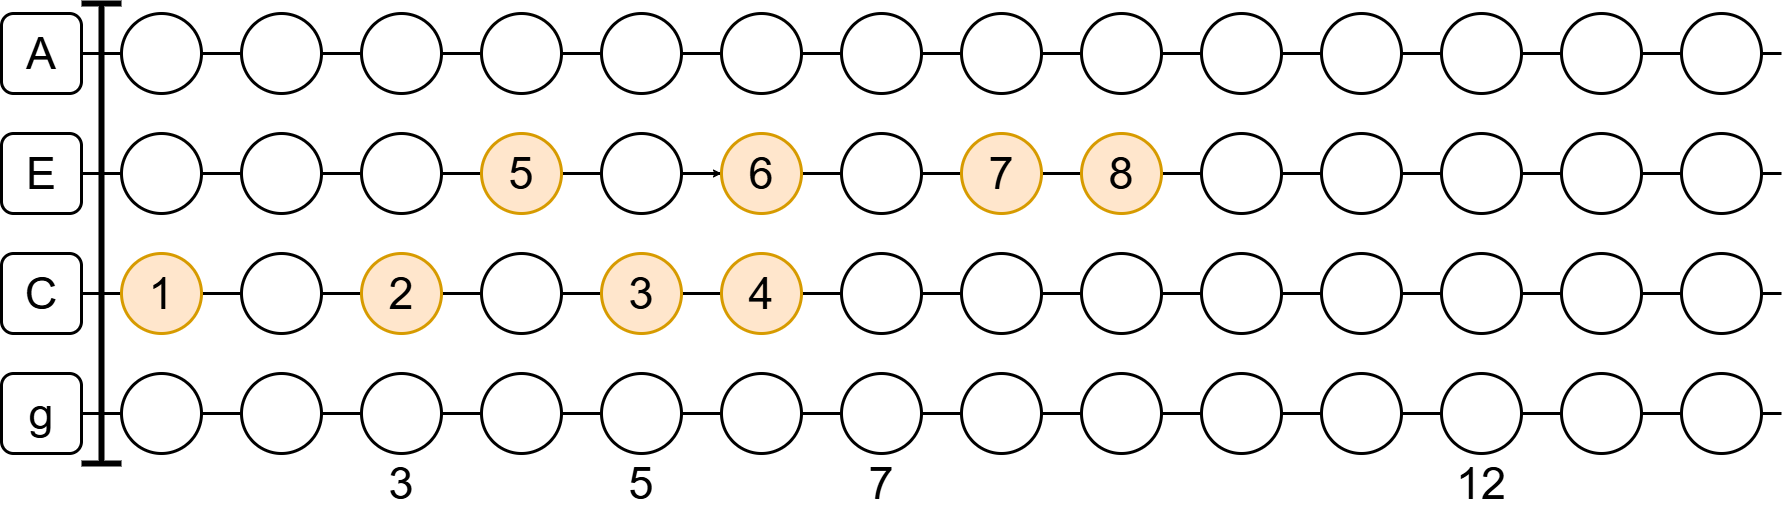
\includegraphics[width=\textwidth]{../../Images/ukulele_major_scale_double_string_from_c.png}
		\caption{Major scale on the fretboard on two strings starting from the C string}
		\label{fig:ukulele_major_scale_fretboard_double_string_from_c}
	\end{subfigure}
	
	\caption{Major scale on the fretboard}
	\label{fig:ukulele_major_scale_fretboard}
\end{figure}

\newpage

Of course, you don't have to start on the C string. you can also start on the E string. Then the two-string shape would look like \autoref{fig:ukulele_major_scale_fretboard_double_string_from_e}. Here we are playing an F major scale.

\begin{figure}[h]
	\centering
	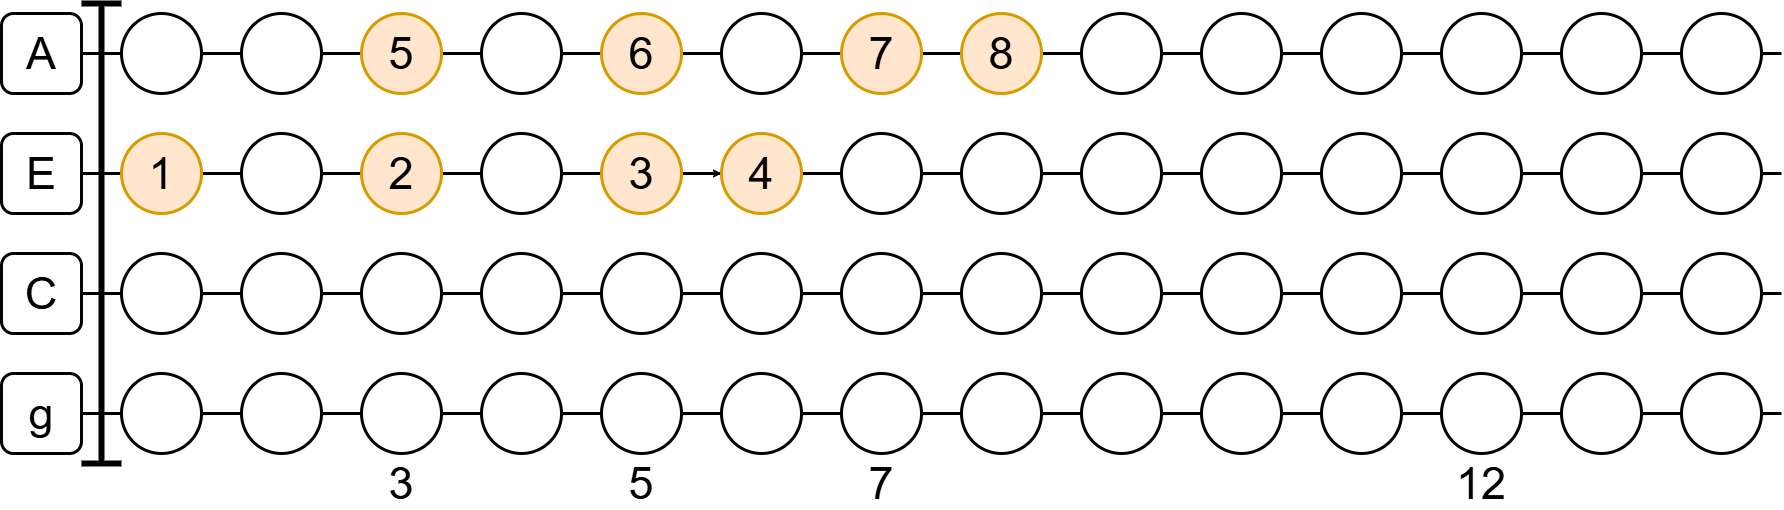
\includegraphics[width=\textwidth]{../../Images/ukulele_major_scale_double_string_from_e.png}
	\caption{Major scale on the fretboard on two strings starting from the E string}
	\label{fig:ukulele_major_scale_fretboard_double_string_from_e}
\end{figure}

Now that we've seen a lot of different ways to play the major scale, we will start focusing on the most compact shape. The shape shown in \autoref{fig:ukulele_major_scale_fretboard_compact}.

\subsubsection{Exercise}

In \autoref{chap:empty_ukulele_fretboard} you see some empty ukulele fretboards. Try to fill these with the different major scales (A, B, C, D, E, F, G) that we've seen in \autoref{tab:ukulele_natural_note_major_scale}. Write the note names instead of the numbers 1-8. Use the shape from \autoref{fig:ukulele_major_scale_fretboard_compact}. You can of course print out the empty ukulele fretboard diagram as often as you want.

While doing this exercise, don't forget to play the scales on the ukulele as well.

% I don't particularly like modes a lot.